%xelatex
\documentclass[14pt]{extreport}

\usepackage[T2A]{fontenc}
\usepackage[utf8]{inputenc}
\usepackage[english,ukrainian]{babel}
\usepackage{amsmath}
\usepackage{mathtools}
\usepackage{caption}
\usepackage{mathspec}
\setallmainfonts{Nimbus Roman}
\usepackage{graphicx}
\usepackage{tikz}
\usetikzlibrary{tikzmark}
\usepackage[a4paper,margin=0.5in]{geometry}
\usepackage{indentfirst}
\usepackage{wrapfig}
\usepackage{subfiles}

\begin{document}
\pagestyle{empty}

\subfile{title}

\subsection*{Мета роботи}

Мета роботи – освоїти методи мінімізації булевих функцій та їх застосування
для оптимізації функціональних схем.
%\begin{center}\bf Варіант 12\end{center}

\subfile{yank.tex}

\newpage
\subsection*{Методом Куайна знайти МДНФ для заданої ДДНФ булевої функції}

$$f_0=xyz\lor\bar xyz\lor\bar x \bar yz\lor x \bar y \bar z \lor\bar xy\bar z$$
$$\hphantom{20pt} 1 \hspace{28pt} 2\hspace{28pt} 3\hspace{28pt} 4\hspace{28pt} 5$$

$1:2- yz$

$2:3- \bar xz$

$2:5- \bar xy$

%3:
%4:

$$f_1=yz\lor\bar xy\lor\bar xz\lor x\bar y\bar z$$

\begin{table}[h]
\centering
\begin{tabular}{|c|c|c|c|c|c|}
	\hline
	& $xyz$ & $\bar xyz$ & $\bar x \bar y z$ &
	$x\bar y\bar z$ & $\bar x y\bar z$\\
	\hline
	$yz$ &\tikzmark{startcore1}\tikzmark{sa}
	\tikzmark{start1}* \tikzmark{endcore1}
	& \tikzmark{se}* &\tikzmark{sb} &\tikzmark{sc} &\tikzmark{end1}\tikzmark{sd}\\
	\hline
	$\bar xy$ &\tikzmark{start2} & * & & &\tikzmark{startcore2} *\tikzmark{endcore2}\tikzmark{end2}\\
	\hline
	$\bar xz$ &\tikzmark{start3} & * &\tikzmark{startcore3} *\tikzmark{endcore3} & & \tikzmark{end3}\\
	\hline
	$x\bar y\bar z$ &\tikzmark{ea}\tikzmark{start4}
	&\tikzmark{ee} &\tikzmark{eb} &\tikzmark{ec}\tikzmark{startcore4} *\tikzmark{endcore4}
	& \tikzmark{end4}\tikzmark{ed}\\
	\hline
\end{tabular}
	\caption{Імплікантна таблиця для СДНФ $f_1$ булевої функціії $f_0$}
\end{table}

\begin{tikzpicture}[remember picture,overlay]
\foreach \Val in {1,2,3,4}
{
\draw[red,thick]
  ([shift={(-12\tabcolsep,1.0ex)}]pic cs:start\Val)
  rectangle
  ([shift={(12\tabcolsep,1.ex)}]pic cs:end\Val);
}

\foreach \Val in {core1,core2,core3,core4}
{
\draw[thick,rounded corners]
  ([shift={(-0.3\tabcolsep,1.7ex)}]pic cs:start\Val)
    rectangle
  ([shift={(0.3\tabcolsep,-0ex)}]pic cs:end\Val);
}

\foreach \Val in {a,b,c,d,e}
{
\draw[thick,violet]
  ([shift={(7pt,1.7ex)}]pic cs:s\Val)
    --
  ([shift={(-0pt,-0ex)}]pic cs:e\Val);
}

\end{tikzpicture}

Викресливши спочатку рядки, де знаходяться імпліканти ядра, а потім
стовпці, в яких є хоча б один викреслений елемент, я виявив,
що функцію більше не можна спростити. Отже,
~$f_1=yz\lor\bar xy\lor\bar xz\lor x\bar y\bar z$
є кінцевим результатом.

\subsection*{Спростити функціональну схему за допомогою карт Карно}
\begin{figure}[h]
	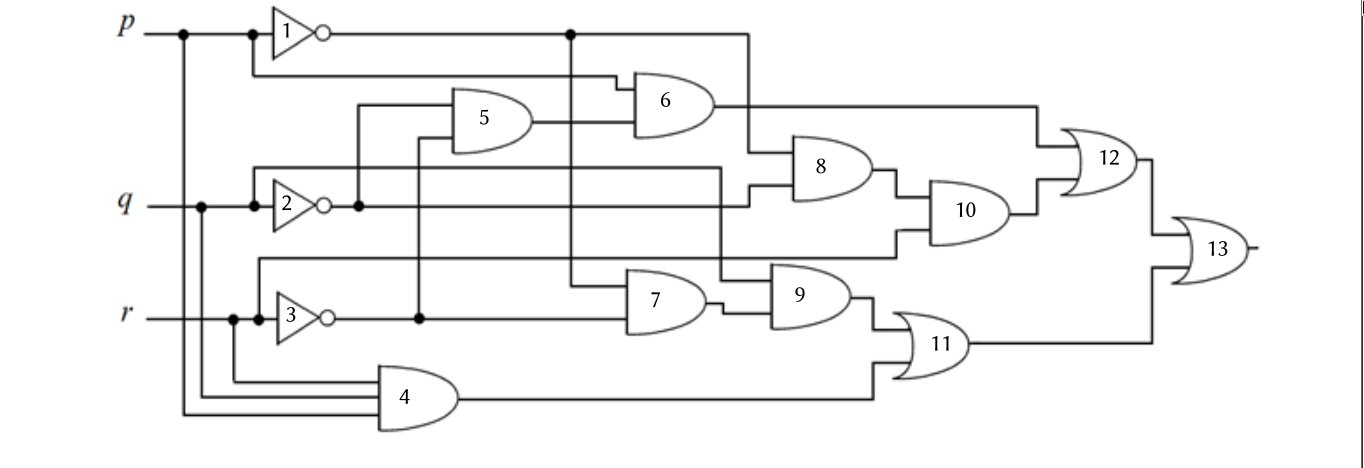
\includegraphics[width=17cm]{es.png}
	\caption{задана функціональна схема}
\end{figure}
\newpage
\begin{table}[h]
	\centering
\begin{tabular}{ccc}
	Вентиль & Вхід & Вихід \\
	\hline
	1 & $p$ & $\bar p$ \\
	\
	2 & $q$ & $\bar q$ \\
	3 & $r$ & $\bar r$ \\
	4 & $p,q,r$ & $pqr$ \\
	5 & $\bar q, \bar r$ & $\bar q\bar r$ \\
	6 & $p,\bar q\bar r$ & $p\bar q\bar r$ \\
	7 & $\bar p, \bar r$ & $\bar p\bar r$ \\
	8 & $\bar p,\bar q$ & $\bar p\bar q$ \\
	9 & $q,\bar p\bar r$ & $q\bar p\bar r$ \\
	10 & $\bar p\bar q,r$ & $\bar p\bar qr$ \\
	11 & $q\bar p\bar r, pqr$ & $q\bar p\bar r\lor pqr $ \\
	12 & $p\bar q\bar r,\bar p\bar qr$ &
	$p\bar q\bar r\lor\bar p\bar qr$ \\
	13 & $q\bar p\bar r\lor pqr,
	p\bar q\bar r\lor\bar p\bar qr$ &
	$(q\bar p\bar r\lor pqr)
	\lor
	(p\bar q\bar r\lor\bar p\bar qr)$ \\
\end{tabular}
\end{table}

Остаточний вигляд функції за схемою:
$$
	\bar pq\bar r\lor pqr
	\lor
	p\bar q\bar r\lor\bar p\bar qr
$$

\begin{table}[h]
	\centering
\begin{tabular}{|c|c|c|c|c|c|}
	\hline
	& $qr$ & $q\bar r$ & $\bar q\bar r$ & $\bar q r$\\
	\hline
	$p$ & x & & x &\\
	\hline
	$\bar p$ & & x &
	 & x \\
	\hline
\end{tabular}
	\caption{}
\end{table}

В таблиці 2 бачимо, що елементів,
які можна об'єднати в контур, немає,
отже, ця функція вже є максимально спрощеною.

\subsection*{Висновок}

Виконуючи цю розрахунково-графічну роботу, я
закріпив уміння знаходити мінімальні диз'юнктивні
нормальні форми булевих функцій методом Куайна та
працювати з функціональними схемами, зокрема
спрощувати їх, використовуючи метод карт Карно.

У першому завданні, виконавши спрощення, я
одразу знайшов мінімальну диз'юн-\\ктивну нормальну форму функції,
виявивши, що більше не зможу мінімізувати її ні за допомогою
операцій неповного склеювання та поглинання, ні з використанням
таблиці.

У другому завданні, проаналізувавши
таблицю, я виявив,
що функцію жодним чином спростити не вдасться.
Подумки застосувавши метод Куайна,
ще раз пересвідчився в цьому. Тому схему залишив
незміненою.

\end{document}
